%!TEX root = maths.tex
\usetikzlibrary{patterns,intersections,arrows,backgrounds}

\newcommand{\degre}{\ensuremath{^\circ}}
\pgfplotsset{compat=1.15}
\usetikzlibrary{arrows}


\graphicspath{pictures/Polar_Curves}
\begin{document}
	\chapter{Polar Curves}
	\section{Introduction}
	The position of a point on a plane can be described in sever ways. With respect to some origin $O$
	we can locate a point $P$ on a plane by noting a horizontal distance followed by a vertical distance.\\
	\definecolor{uququq}{rgb}{0.25,0.25,0.25}
	\definecolor{xdxdff}{rgb}{0.49,0.49,1}
	\definecolor{qqqqff}{rgb}{0,0,1}
	\definecolor{xdxdff}{rgb}{0.49,0.49,1}
	\definecolor{qqqqff}{rgb}{0,0,1}
	\begin{center}
		\definecolor{xdxdff}{rgb}{0.49,0.49,1}
		\definecolor{qqqqff}{rgb}{0,0,1}
		\begin{tikzpicture}[line cap=round,line join=round,>=triangle 45,x=1.0cm,y=1.0cm]
		\draw[->,color=black] (-1,0) -- (5,0);
		\foreach \x in {-1,1,2,3,4}
		\draw[shift={(\x,0)},color=black] (0pt,2pt) -- (0pt,-2pt) node[below] {\footnotesize $\x$};
		\draw[->,color=black] (0,-1) -- (0,4);
		\foreach \y in {-1,1,2,3}
		\draw[shift={(0,\y)},color=black] (2pt,0pt) -- (-2pt,0pt) node[left] {\footnotesize $\y$};
		\draw[color=black] (0pt,-10pt) node[right] {\footnotesize $0$};
		\clip(-1,-1) rectangle (5,4);
		\draw [dash pattern=on 1pt off 1pt] (0,3)-- (4,3);
		\draw [dash pattern=on 1pt off 1pt] (2.08,3) -- (2,2.9);
		\draw [dash pattern=on 1pt off 1pt] (2.08,3) -- (2,3.1);
		\draw [dash pattern=on 1pt off 1pt] (4,0)-- (4,3);
		\draw [dash pattern=on 1pt off 1pt] (4,1.58) -- (4.1,1.5);
		\draw [dash pattern=on 1pt off 1pt] (4,1.58) -- (3.9,1.5);
		\begin{scriptsize}
		\fill [color=red] (4,3) circle (1.5pt);
		\draw[color=black] (4.31,3.19) node {$P$ ($x$, $y$)};
		\fill [color=qqqqff] (4,0) circle (1.5pt);
		\draw[color=black] (4.2,0.2) node {$X$};
		\fill [color=qqqqff] (0,3) circle (1.5pt);
		\draw[color=black] (0.2,3.19) node {$Y$};
		\end{scriptsize}
		\end{tikzpicture}
	\end{center}
	
	However the point $P$ can be located on a plane with respect to the origin $O$, a horizontal line and the distance of $P$ from $O$.\\
	
	\definecolor{ttttff}{rgb}{0.2,0.2,1}
	\definecolor{qqqqff}{rgb}{0,0,1}
	\definecolor{cqcqcq}{rgb}{0.75,0.75,0.75}
	\definecolor{ttttff}{rgb}{0.2,0.2,1}
	\definecolor{qqqqff}{rgb}{0,0,1}
	\begin{center}
		
		\begin{tikzpicture}[line cap=round,line join=round,>=triangle 45,x=1.0cm,y=1.0cm]
		\draw[->,color=black] (-1,0) -- (6,0);
		\foreach \x in {-1,1,2,3,4,5}
		\draw[shift={(\x,0)},color=black] (0pt,2pt) -- (0pt,-2pt) node[below] {\footnotesize $\x$};
		\draw[->,color=black] (0,-1) -- (0,6);
		\foreach \y in {-1,1,2,3,4,5}
		\draw[shift={(0,\y)},color=black] (2pt,0pt) -- (-2pt,0pt) node[left] {\footnotesize $\y$};
		\draw[color=black] (0pt,-10pt) node[right] {\footnotesize $0$};
		\clip(-1,-1) rectangle (6,6);
		\draw [shift={(0,0)},color=ttttff,fill=ttttff,fill opacity=0.1] (0,0) -- (0:0.71) arc (0:45:0.71) -- cycle;
		\draw (0,0)-- (3,3);
		\begin{scriptsize}
		\fill [color=qqqqff] (0,0) circle (1.5pt);
		\draw[color=black] (-0.4,-0.3) node {Pole};
		\fill [color=red] (3,3) circle (1.5pt);
		\draw[color=black] (3.52,3.21) node {$P$ ($r$, $\theta$)};
		\draw[color=black] (1.71,1.44) node {$r$};
		\draw[color=black] (0.46,0.2) node {$\theta$};
		\end{scriptsize}
		\end{tikzpicture}
		
	\end{center}
	
	This is the polar coordinate system where we refer to the origin as the pole and the horizontal line as the initial line. The anti clockwise angle is usually measured in the principal range $-\pi < \theta \leq \pi$.
	\newpage
	\section{Relationship between Polar and Cartesian Coordinates}
	
	Consider the following diagram showing the point P on the plane, both in Cartesian and Polar coordinates
	
	The above relationship can be used to convert from one form to another.
	\begin{example}
		Find the polar coordinates of the curve given by $y=x^2+y^2=2x$
	\end{example}
	
	\begin{alignat*}{2}
	& \qquad \quad x^2+y^2  &   & = 2x  \\    
	& \implies 2r\cos\theta &   & = r^2 \\
	& \implies 2\cos\theta  &   & = r   
	\end{alignat*}
	
	
	\hrulefill
	\begin{example}
		Find the Cartesian equation corresponding to the curves \textbf{a)} $r=4(1+\cos\theta)$ and \textbf{b)} $3 = r\sin 2\theta$.
	\end{example}
	\begin{equation*}
	\begin{split}
	r &= 4(1+\cos\theta)
	\end{split}
	\qquad \qquad \qquad
	\begin{split}
	3 &= r\sin2\theta\\
	3 &= 2r\sin\theta\cos\theta\\	
	3  &= 2x\sin\frac yr
	\end{split}
	\end{equation*}
	$$i^2 + 1^2 = 0$$
	
	\newpage
	\section{Sketching Polar Curves}
	\begin{example}
		Sketch the polar curve of $2+2\cos\theta$.
	\end{example}
	Observing the following sketch, it is shown that a line of symmetry is present in the $x$-axis for the \emph{cosine} function family.
	\begin{center}
		\resizebox{300pt}{!}{%
			\begin{tabular}{c|c|c|c|c|c|c|c|c|c}
				
				$\displaystyle\theta$ & $0$ & $\frac\pi6$ & $\frac\pi4$ & $\frac\pi3$ & $\frac\pi2$ & $\frac{2\pi}3$ & $\frac{3\pi}4$ & $\frac{5\pi}6$ & $\pi$ \\ \hline
				$r$                   & 4   & 3.7         & 3.4         & 3           & 2           & 1              & 0.6            & 0.3            & 0     
			\end{tabular}
		}
	\end{center}
	\begin{center}
		\begin{tikzpicture}[scale=1.7]
		\draw[thick,->,>=latex] (-3,0)--(5,0) node[above] {$x$};
		\draw[thick,->,>=latex] (0,-3)--(0,4) node[left] {$y$};
		\draw[domain=0:540,scale=1,samples=1000] plot (\x:{2+(2*cos(\x))});
		\clip (-3,-3) rectangle (6,4);
		
		% Draw dotted lines and crosses
		\foreach \i in {0, {pi/6},{pi/4}, {pi/3}, {2* pi / 3}, {3 * pi / 4}, {5 *pi / 6}, {pi}}{
			\draw[red, dashed, samples=500] plot(\x, {tan( deg(\i)) * \x});
			\pic[line width=1pt,green] at ({deg(\i)}:{2+(2*cos(deg(\i)))}) {mycross};}																																		
		\end{tikzpicture}
	\end{center}
	\newpage
	\begin{example}
		Sketch the graph with polar equation $r=3-2\cos\theta$.
	\end{example}
	Similarly to the above example, a line of symmetry is present in the $x$-axis.
	\begin{center}
		\resizebox{300pt}{!}{%
			\begin{tabular}{c|c|c|c|c|c|c|c|c|c}
				$\displaystyle\theta$ & $0$ & $\frac\pi6$ & $\frac\pi4$ & $\frac\pi3$ & $\frac\pi2$ & $\frac{2\pi}3$ & $\frac{3\pi}4$ & $\frac{5\pi}6$ & $\pi$ \\ \hline
				$r$                   & 1   & 1.3         & 1.6         & 2           & 3           & 4              & 4.4            & 4.7            & 5     
			\end{tabular}
		}
	\end{center}
	
	
	
	\begin{center}
		\begin{tikzpicture}
		\draw[thick,->,>=latex] (-6,0)--(4,0) node[above] {$x$};
		\draw[thick,->,>=latex] (0,-4)--(0,4) node[left] {$y$};
		\draw[domain=0:540,scale=1,samples=500] plot (\x:{3-(2*cos(\x))});
		\clip (-5,-5) rectangle (6,4);
		
		%	Draw dotted lines and crosses
		\foreach \i in {0, {pi/6},{pi/4}, {pi/3}, {2* pi / 3}, {3 * pi / 4}, {5 *pi / 6}, {pi}}{
			\draw[red, dashed, thick, samples=500] plot(\x, {tan( deg(\i)) * \x});
			\pic[line width=1pt,green] at ({deg(\i)}:{3-(2*cos(deg(\i)))}) {mycross};}
		\end{tikzpicture}
	\end{center}
	\newpage
	\begin{example}
		Sketch the graph with polar equation $r=5+2\sin\theta$.
	\end{example}
	
	It is noted that since the graph is part of the \emph{sine} function family,the line of symmetry is now present in the $y$-axis.
	
	\begin{center}
		\resizebox{300pt}{!}{%
			\begin{tabular}{c|c|c|c|c|c|c|c|c|c}
				$\theta$ & $\frac{-\pi}2$ & $\frac{-\pi}3$ & $\frac{-\pi}4$ & $\frac{-\pi}6$ & 0   & $\frac\pi6$ & $\frac\pi4$ & $\frac\pi3$ & $\frac\pi2$ \\ \hline
				$r$      & 3              & $3.3$          & $3.6$          & $4$            & $5$ & $6$         & $6.4$       & $6.7$       & $7$         
			\end{tabular}
		}
	\end{center}
	
	\begin{center}
		\begin{tikzpicture}
		\draw[thick,->,>=latex] (-8,0)--(6,0) node[above] {$x$};
		\draw[thick,->,>=latex] (0,-4)--(0,9) node[left] {$y$};
		\draw[domain=0:540,scale=1,samples=500] plot (\x:{5+(2*(sin(\x)))});
		
		\clip (-9,-4) rectangle (8,8);
		
		%	Draw dotted lines and crosses
		\foreach \i in {{-pi/6},{-pi/4}, {-pi/3}, 0, {pi/6},{pi/4}, {pi/3}}{
			\draw[red, dashed, thick, samples=500] plot(\x, {tan( deg(\i)) * \x});
			\pic[line width=1pt,green] at ({deg(\i)}:{5+(2*(sin(deg(\i))))}) {mycross};}
		\end{tikzpicture}
	\end{center}
	
	\newpage
	\begin{example}
		Sketch the polar curve $r=3+7\sin\theta$ and the circle $r=5$. Find the polar coordinates of their points of intersection.
	\end{example}
	
	\begin{center}
		\begin{tikzpicture}
		\draw[thick,->,>=latex] (-7,0)--(7,0) node[above] {$x$};
		\draw[thick,->,>=latex] (0,-6)--(0,11) node[left] {$y$};
		\draw[domain=0:540,scale=1,samples=1000] plot (\x:{3+(7*sin(\x))}); %Curve
		\draw[domain=0:540,scale=1,samples=500] plot (\x:5);				%Circle
		\clip (-7,-2) rectangle (6,10);
		
		%Draw dotted lines and crosses
		\foreach \i in {{-pi/6},{-pi/4}, {-pi/3}, 0, {pi/6},{pi/4}, {pi/3}}{
			\draw[red, dashed, thick, domain=-7:7, samples=500] plot(\x, {tan( deg(\i)) * \x});
			\pic[line width=1pt,green] at ({deg(\i)}:{3+(7*sin(deg(\i)))}) {mycross};}
		
		\draw[red, dashed, thick, domain=-7:12, samples=500] plot(0,\x);
		%Tangential Asymptotes
		\pic[line width=1pt,green] at ({deg(pi/2)}:10) {mycross};
		\pic[line width=1pt,green] at ({deg(-pi/2)}:-4) {mycross};
		
		\end{tikzpicture}
	\end{center}
	
	
	\newpage
	\begin{example}
		Sketch the polar curve $r=8\sin^2\theta$ and the line $r=\csc\theta$. Find the polar coordinates of their points of intersection.
	\end{example}
	\begin{center}
		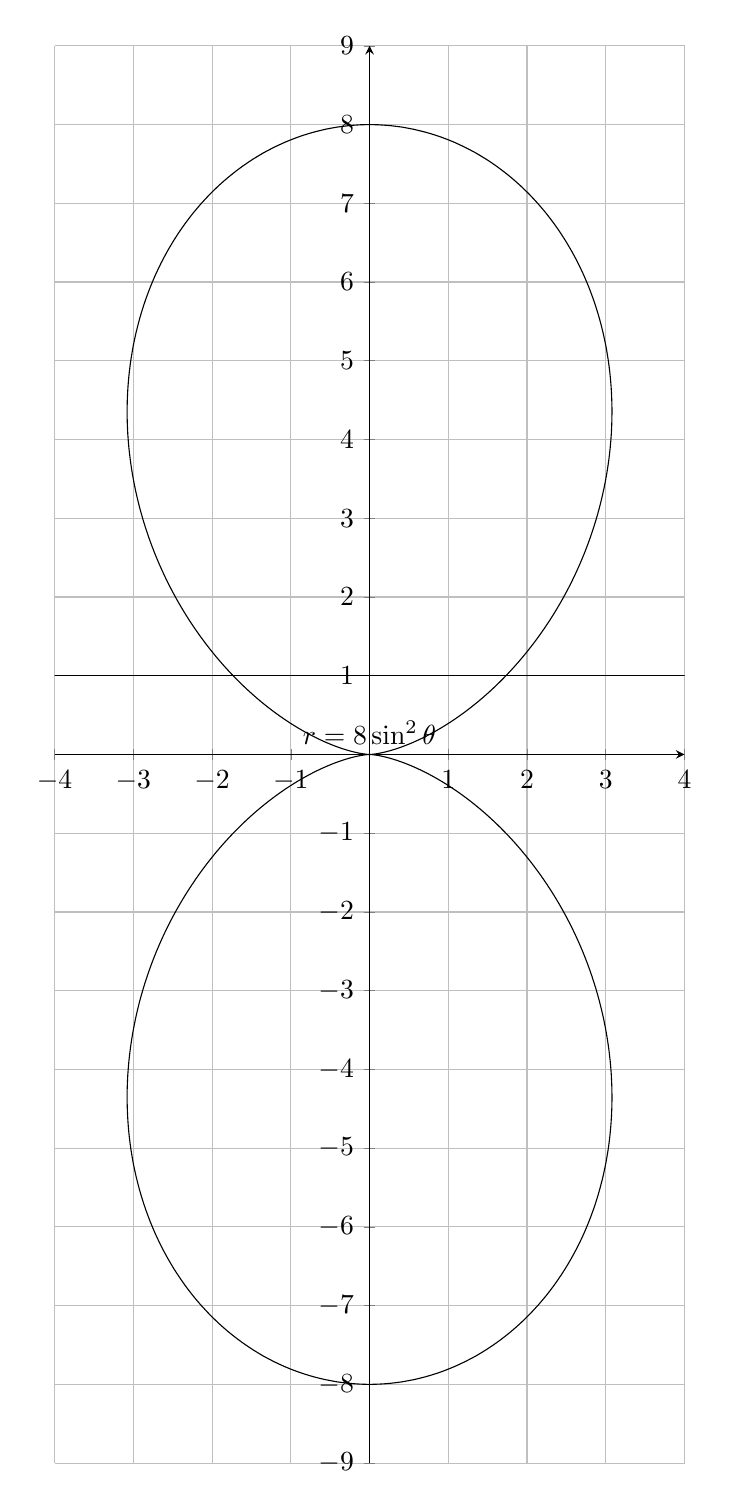
\begin{tikzpicture}
			\begin{axis}[
			x=1cm,y=1cm,
			axis lines=middle,
			ymajorgrids=true,
			xmajorgrids=true,
			xmin=-4,
			xmax=4,
			ymin=-9,
			ymax=9,
			xtick={-4,-3,...,4},
			ytick={-9,-8,...,9},]
		\draw[domain=0:540,scale=1,samples=1000] plot (\x:{8*(sin(\x)^2)}) node[above] {$r=8\sin^2\theta$}; %Curve
		\draw[domain=-5:5,scale=1,samples=1000] plot (\x, 1) node[above] {$r=\csc\theta$}; %Curve
	%	\clip (-7,-2) rectangle (6,10);
\end{axis}
		\end{tikzpicture}
	\end{center}

\section{Area partly bounded by a polar curve}
Consider the following diagram showing the graph of $r=f(\theta)$.

\begin{center}
	\resizebox{300pt}{!}{%
	\definecolor{ccffww}{rgb}{0.8,1,0.4}
	\definecolor{qqttcc}{rgb}{0,0.2,0.8}
	\definecolor{uuuuuu}{rgb}{0.26666666666666666,0.26666666666666666,0.26666666666666666}
	\definecolor{xdxdff}{rgb}{0.49019607843137253,0.49019607843137253,1}
	\begin{tikzpicture}[line cap=round,line join=round,>=triangle 45,x=1cm,y=1cm]
		\begin{axis}[
			x=1cm,y=1cm,
			axis lines=middle,
			ymajorgrids=true,
			xmajorgrids=true,
			xmin=-4.087350135407929,
			xmax=12.075704876608706,
			ymin=-1.9400069331551724,
			ymax=8.089791136292845,
			xtick={-4,-3,...,12},
			ytick={-1,0,...,8},]
			\clip(-4.087350135407929,-1.9400069331551724) rectangle (12.075704876608706,8.089791136292845);
			\draw [shift={(0,0)},line width=2.4pt,color=qqttcc,fill=qqttcc,fill opacity=0.1] (0,0) -- (27.797567846322046:0.9614841741650471) arc (27.797567846322046:72.69166717480417:0.9614841741650471) -- cycle;
			\fill[line width=0.8pt,color=ccffww,fill=ccffww,fill opacity=0.55] (1.6469997622170334,5.285200045490499) -- (1.8018963690587861,5.303857839349265) -- (2.057802642713001,5.344452622890168) -- (2.2425420008780867,5.375610046949744) -- (2.4085986469696503,5.401170598203379) -- (2.6317350137162325,5.427157717856224) -- (2.826543364850297,5.438046959825773) -- (2.9930508460166525,5.436092904437624) -- (3.1583701235903847,5.422111858769122) -- (3.394065928081652,5.378740328890088) -- (3.5780745473050493,5.323957494370168) -- (3.7684491850962933,5.246759511526517) -- (3.909043353636018,5.175946821869229) -- (4.096867913840399,5.062840104074621) -- (4.339673854011711,4.885528774754539) -- (4.70860996427174,4.552297629385634) -- (5.130951567039364,4.088855310480258) -- (5.420878217861827,3.7324711921147538) -- (5.752127039672099,3.3035617372125) -- (5.8996282307282275,3.1102010591021587) -- (0,0) -- cycle;
			\draw [line width=2pt,dash pattern=on 1pt off 1pt,domain=-4.087350135407929:12.075704876608706] plot(\x,{(-0--4.099788120747726*\x)/1.2775959286106953});
			\draw [line width=2pt,dash pattern=on 1pt off 1pt,domain=-4.087350135407929:12.075704876608706] plot(\x,{(-0--4.87618*\x)/9.24945});
			\draw[line width=2pt,color=xdxdff,smooth,samples=100,domain=-4.087350135407929:12.075704876608706] plot(\x,{0.014635180803888441*(\x)^(4)-0.23126329831793696*(\x)^(3)+1.0699408938350827*(\x)^(2)-1.8059409257011467*(\x)+6.282771603030379});
			\draw (2.6126764256158723,7.846889871240623) node[anchor=north west] {$\large \theta = \alpha$};
			\draw (7.440339068528793,5.195217727753861) node[anchor=north west] {$\large \theta = \beta$};
			\draw [color=xdxdff](-2.5287336846561685,8.960187336063308) node[anchor=north west] {$\large r=f({\theta})$};
			\begin{scriptsize}
				\draw [fill=uuuuuu] (1.6469997622170334,5.285200045490499) circle (2pt);
%				\draw[color=uuuuuu] (1.74734066886733,5.524146524178746) node {$G$};
				\draw [fill=uuuuuu] (0,0) circle (2pt);
				\draw [fill=uuuuuu] (5.8996282307282275,3.1102010591021587) circle (2pt);
				\draw[color=uuuuuu] (6.038596351456593,3.3937000119498784) node {$D_1$};
				\draw[color=qqttcc] (1.0743017469517973,0.5143079324766583) node {$\Large\omega$};
			\end{scriptsize}
		\end{axis}
	\end{tikzpicture}
}
\end{center}
It can be shown that the area bounded by the curve $r=f(\theta)$, from $\theta = \alpha$ to $\theta = \beta$ is given by \[A = \frac12\int_\alpha^\beta r^2\,d\theta\]
\hrulefill
\begin{example}
	Sketch the curve with polar equation $r=2(1-\cos\theta)(\sqrt{\sin\theta})$ for $0 \leq \theta\leq \pi$ and find the area it encloses.
\end{example}
\begin{center}
\begin{tabular}{c|c|c|c|c|c|c|c|c|c|c|c|c|c}
	$\theta$ & 0                     & $\frac{\pi}{12}$      & $\frac{\pi}6$         & $\frac{\pi}4$         & $\frac{\pi}3$         & $\frac{5\pi}{12}$     & $\frac\pi2$           & $\frac{7\pi}{12}$     & $\frac{2\pi}3$        & $\frac{3\pi}4$        & $\frac{5\pi}6$        & $\frac{11\pi}{12}$    & $\pi$                \\ \hline
	$r$      & $0$                   & $0.03$                & $0.2$                   & $0.5$                   & $0.9$                   & $1.5$                   & $2$                   & $2.5$                 & $11$                 & $2.9$                 & $2.6$                 & $2$                     & $0$
\end{tabular}
\end{center}
	\begin{center}
	\begin{tikzpicture}
\begin{axis}[
x=1cm,y=1cm,
axis lines=middle,
ymajorgrids=true,
xmajorgrids=true,
xmin=-4,
xmax=4,
ymin=-4,
ymax=4,
xtick={-4,-3,...,4},
ytick={-4,-3,...,4},]
\coordinate (origin) at (0,0);
\end{axis}
\begin{scope}[shift={(origin)}]
		\clip (-4,-4) rectangle (4,4);
\draw[domain=0:180,scale=1,samples=500 ] plot (\x:{2*(1-cos(\x))*(sqrt(sin(\x))) }); %Curve 

	\foreach \i in {0,15,...,75,105,120,...,180}{
	\draw[red, dashed, thick, domain=-5:5, samples=500] plot(\x, {tan(\i) * \x});
	\pic[line width=1pt,green] at ({\i}:{2*(1-cos(\i))*(sqrt(sin(\i))) }) {mycross};
}
		\draw[red, dashed, thick, domain=-5:5, samples=500] plot(0,\x);
	\pic[line width=1pt,green] at (0,2) {mycross};	
\end{scope}
	
		

	\end{tikzpicture}
\end{center}
\end{document}
